\section{Introduction}
    In the Vortex \ae ther Model (VAM), gravitation and quantum phenomena are reformulated through the topology and dynamics of vorticity in an incompressible, inviscid fluid-like \ae ther. This article derives a formal connection between classical defect theory---dislocations and disclinations in condensed matter physics---and VAM's vortex core structures using the language of Cartan geometry. Inspired by recent developments \cite{kobayashi2025}, we reinterpret torsion and curvature within the Cartan structure equations in terms of swirl density and topological vortex curvature. Furthermore, we show that light itself---the photon---can be interpreted as a topologically stable vortex ring, unifying electromagnetic energy propagation with the mechanics of superfluid circulation.
    We aim to bridge the gap between the abstract formalism of QED and the physical intuition of light as a structured entity by modeling the photon as a quantized vortex ring. This yields testable predictions for polarization-dependent birefringence and modified vortex interaction cross-sections in structured vacua.


\section{Vortex Ring and Cartan Torsion}

\begin{center}
    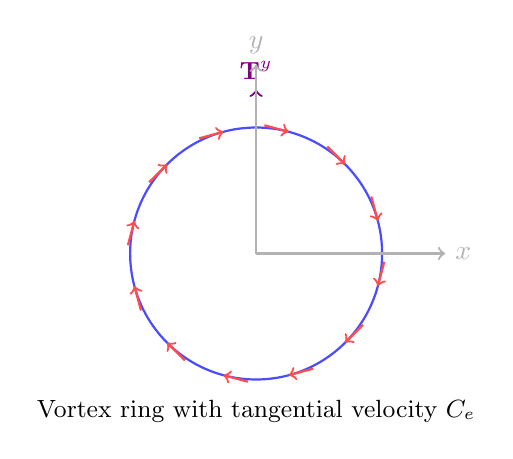
\begin{tikzpicture}[scale=0.8]
        % Ring (vortex core)
        \draw[thick, blue!70] (0,0) circle (2);

        % Flow lines (tangential swirl)
        \foreach \a in {15,45,75,105,135,165,195,225,255,285,315,345} {
            \draw[->, red!70, thick]
            ({2*cos(\a)}, {2*sin(\a)})
            ++({-0.4*sin(\a)}, {0.4*cos(\a)})
            -- ++({0.4*sin(\a)}, {-0.4*cos(\a)});
        }

        % Central torsion arrow
        \draw[->, thick, violet] (0,0) -- (0,2.6) node[above] {\small $\mathbf{T}^y$};

        % Axis labels
        \draw[->, thick, gray!60] (0,0) -- (3,0) node[right] {$x$};
        \draw[->, thick, gray!60] (0,0) -- (0,3) node[above] {$y$};

        % Label
        \node at (0,-2.5) {\small Vortex ring with tangential velocity $C_e$};
    \end{tikzpicture}
\end{center}


\noindent
This diagram shows a vortex ring in the $x$-$y$ plane with tangential swirl velocity (red arrows) and central torsion aligned along the $y$-axis,
representing $\mathbf{T}^y$ from Cartan's torsion 2-form.

\begin{figure}[H]
    \centering
    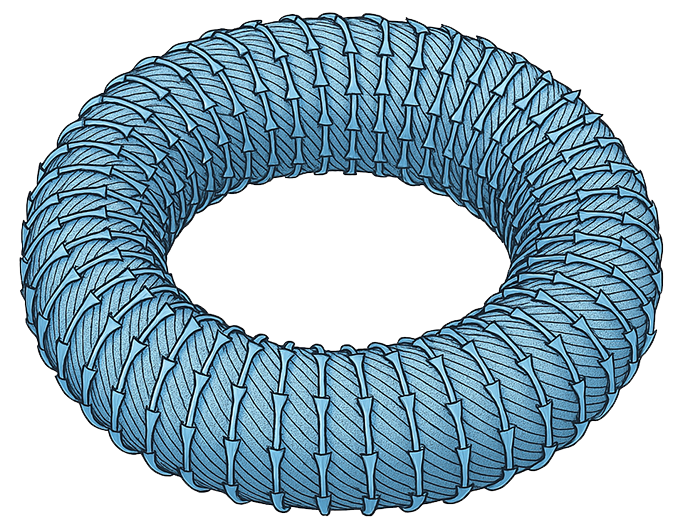
\includegraphics[width=0.9\textwidth]{figures/Un-Knot}
    \caption{Unknotted vortex ring with helically wound circulation — VAM model of a photon. Its topological class is trivial (unknot), corresponding to zero rest mass and helicity-1. Its propagation always satisfies:
        \[
            v = c, \quad \text{with } dt = dt_{\infty}
        \]
        since it experiences no time dilation in the æther. This is consistent with Maxwellian wave propagation as a swirl structure~\cite{maxwell1875}.}
    \label{fig:un-knot}
\end{figure}

\begin{figure}[H]
    \centering
    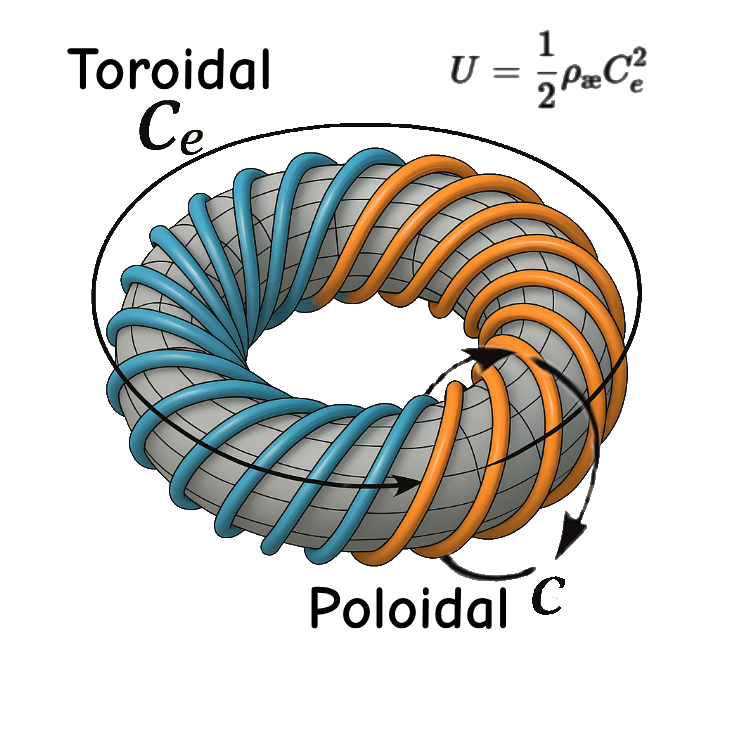
\includegraphics[width=0.25\textwidth]{figures/vortex-fine-structure}
    \caption{
        This dual-motion structure serves as the foundation for modeling photons as stable, knotted æther vortices in VAM.
        Dual-scale vortex winding with toroidal and poloidal circulations. The toroidal circulation speed is $C_e$, while the poloidal component reaches $c$ due to maximum vortex ring propagation. The two scales form a helicity product:
        \[
            \mathcal{H} = \int \vec{v} \cdot \vec{\omega} \, dV \sim \Gamma_{\text{toroidal}} \cdot \Gamma_{\text{poloidal}}
        \]
        This product contributes to the derivation of the fine-structure constant $\alpha$ in VAM~\cite{iskandarani2025b}.
    }
    \label{fig:vortex-3d}
\end{figure}







\begin{figure}[H]
    \centering
    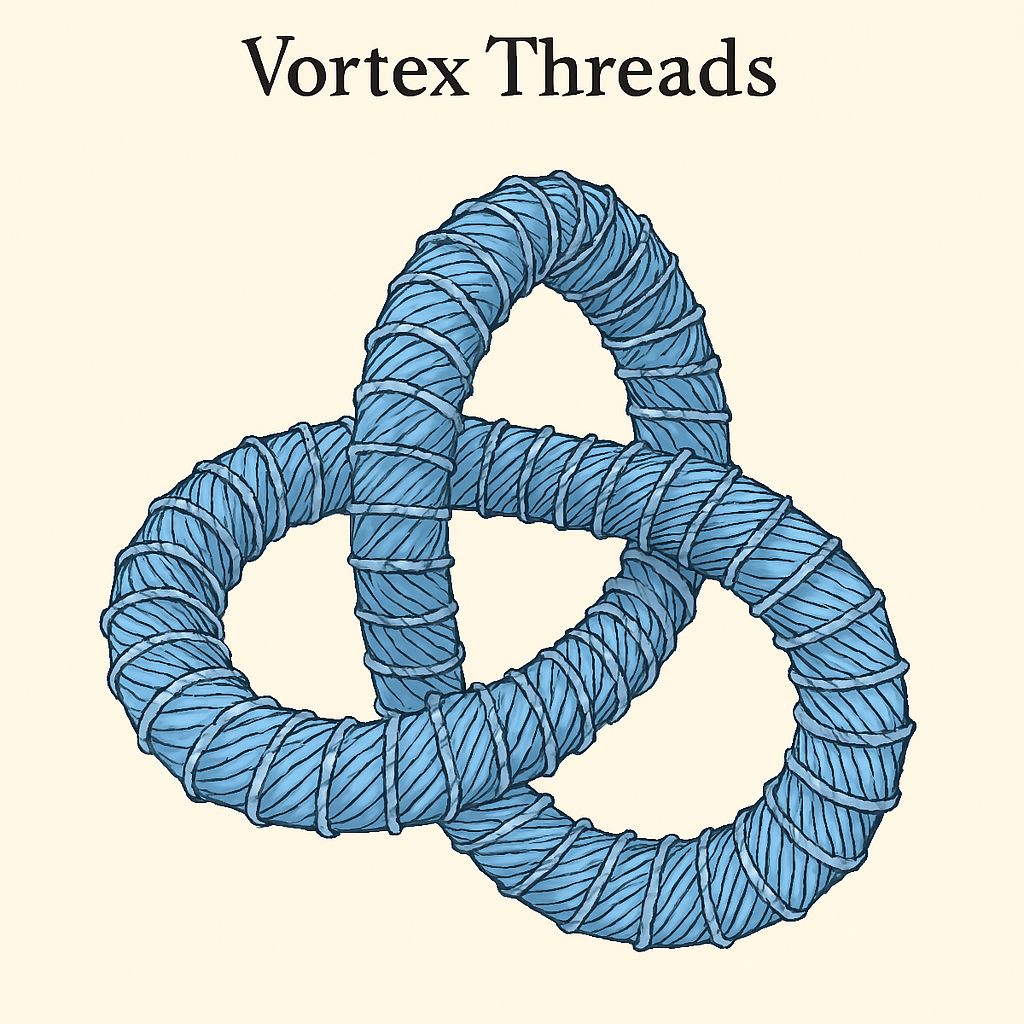
\includegraphics[width=0.35\textwidth]{figures/Tre-foil}
    \caption{Trefoil knot vortex structure — minimal topologically nontrivial knot with chirality. This diagram represents a fermion in VAM (e.g., electron), whose mass is generated from internal knotted swirl energy:
        \[
            m_e \approx \frac{1}{\varphi} \cdot \frac{4}{\alpha} \cdot \left( \frac{1}{2} \rho_{\text{\ae}}^{\text{(energy)}} C_e^2 V \right)
        \]
        where $V$ is the knot volume, $\varphi$ the golden ratio, and $\rho_{\text{\ae}}^{\text{(energy)}}$ the æther energy density~\cite{iskandarani2025a, iskandarani2025b}. This configuration also exhibits chirality, fundamental for distinguishing matter vs antimatter in VAM.}
    \label{fig:trefoil-vortex}
\end{figure}

\section{Related Work and Historical Context}

    The idea of a structured medium underpinning physical phenomena has deep historical roots. Lord Kelvin and Helmholtz first proposed vortex atom models~\cite{thomson1867}, attempting to derive material properties from knotted fluid structures. Maxwell~\cite{maxwell1861} and Lorentz~\cite{lorentz1904} further developed mechanical æther models to explain electromagnetism, before Einstein's relativity discouraged a privileged reference frame.

    Contemporary approaches have revisited these ideas under new lights. In analogue gravity, Unruh~\cite{unruh1981} and Barceló et al.~\cite{barcelo2011} demonstrated that perturbations in a moving fluid obey effective relativistic wave equations, giving rise to phenomena like horizon analogs and Hawking radiation. Volovik~\cite{volovik2003} extended this to quantum fluids, proposing that all fields and metrics may arise from low-energy excitations in a condensed background.

    In photonics, topological concepts have flourished. Lu et al.~\cite{lu2014} and Ozawa et al.~\cite{ozawa2019} showed that photonic crystals and metamaterials can simulate topological phases, suggesting deep connections between light, geometry, and protected vortex-like modes. These developments resonate strongly with the VAM perspective, where photons are topologically stable vortex excitations in a real fluid medium.

    Unlike purely analogue models, VAM posits that the æther is not merely an emergent description but a physically real medium, with its own fundamental properties. In this sense, the model revives and modernizes early æther theories while remaining consistent with relativistic symmetry—much like how effective field theories respect renormalization group invariance without requiring spacetime fundamentalism.

    \begin{quote}
        \emph{VAM bridges 19th-century æther mechanics with 21st-century topological and analogue models, offering a unified fluid-dynamical foundation for matter and radiation.}
    \end{quote}


\section{Historical Roots of the Vortex \ae ther Concept}


    The Vortex \ae ther Model (VAM) is deeply rooted in 19th-century developments in fluid dynamics and early field theory. The historical context reveals that many foundational ideas—long before the emergence of modern quantum field theory—foreshadowed a vortex-based structure of matter and interactions.


    \subsection{Helmholtz and the Birth of Vorticity}


    In 1858, Hermann von Helmholtz laid the foundations of vortex dynamics in his seminal paper on the conservation of vorticity in ideal fluids \cite{helmholtz1858}. He proved that vortex lines in an inviscid, incompressible fluid behave as conserved topological structures and cannot end within the fluid—an idea mirrored in VAM's treatment of knotted particle structures. Helmholtz’s laws implied that such vortices could remain stable indefinitely and interact through their induced velocity fields.


    \subsection{Kelvin's Vortex Atom Hypothesis}


    Building upon Helmholtz’s results, William Thomson (Lord Kelvin) proposed in 1867 that atoms might be understood as knotted vortex rings in the luminiferous \ae ther \cite{kelvin1867}. These vortex atoms were hypothesized to have distinct identities based on their topological class, such as knots and links—ideas that prefigure VAM’s classification of elementary particles. While ultimately overshadowed by the rise of atomic theory, Kelvin’s insight was remarkably prescient.


    \subsection{Maxwell and Mechanical Models of the \ae ther}


    James Clerk Maxwell, in developing his equations for electromagnetism, repeatedly emphasized the need for a mechanical model of the field. In his 1875 work \cite{maxwell1875}, he described an elastic medium with vortical cells and velocity circulation as necessary for maintaining displacement current—a physical concept aligned with the vorticity fields in VAM. Maxwell even referred to angular momentum of field lines as potential carriers of radiation.


    \subsection{Tait and Topological Quantization}


    Peter Guthrie Tait, a close collaborator of Kelvin, extended the mathematical analysis of vortex knots and linked structures. He introduced knot invariants and classifications that echo modern quantum numbers. In VAM, such topological invariants map directly onto conserved quantities like charge, spin, and mass—reviving Tait’s program in a physically rigorous framework.


    \subsection{Modern Revival Through Superfluid Analogues}


    While classical \ae ther theory fell out of favor after the Michelson–Morley experiment, 20th and 21st-century developments in superfluid helium, Bose–Einstein condensates, and topological fluid mechanics have re-energized the field. The VAM integrates these insights while restoring a physically grounded, Euclidean \ae ther with absolute time—aligned with Helmholtz’s and Kelvin’s original vision, but equipped with the mathematical formalism of Cartan geometry and topological field theory.


    \begin{quote}

    \textit{“The vortex theory, though abandoned, left behind the powerful idea that topological structure could be the key to the quantum.”} \[0.5em]

    \hfill -- Helmholtz–Kelvin–Tait lineage, revisited.

    \end{quote}


\section{Physical Interpretation of the Æther}\label{sec:aether-interpretation}

    In the Vortex \ae ther Model (VAM), the \ae ther is a physically real, incompressible, inviscid superfluid that fills all space and serves as the medium in which vortex structures propagate. Unlike the luminiferous æther of pre-relativistic physics, the VAM æther is not a rigid or preferred frame in the classical sense, but a \emph{relational fluid substrate} whose dynamics obey local conservation laws and whose properties are encoded in geometric field variables such as vorticity $\vec{\omega}$, swirl potential $\chi$, and pressure gradients $\nabla P$.

    \subsection{Æther and Relativity}

        Contrary to historical objections (e.g., Michelson--Morley), the VAM æther is consistent with observed relativistic invariance. In VAM:

        \begin{itemize}
            \item The speed of light $c$ emerges as the limiting swirl propagation velocity in the æther.
            \item Time dilation and length contraction are derived from local swirl energy density~\cite{iskandarani2025b}, not from coordinate transformations.
            \item There is no global rest frame detectable through mechanical means, since only \emph{local} vorticity gradients affect physical observables.
        \end{itemize}

        This formulation parallels “emergent spacetime” scenarios in analogue gravity~\cite{barcelo2011}, where effective relativistic metrics arise from fluid microdynamics.

    \subsection{Æther as a Relational Fluid}

        The VAM æther is defined by its core properties:
        \begin{itemize}
            \item \textbf{Incompressibility:} $\nabla \cdot \vec{v} = 0$
            \item \textbf{Inviscid Dynamics:} No intrinsic dissipation; supports persistent circulation.
            \item \textbf{Vortex-Centric Ontology:} All matter, radiation, and fields emerge as stable or propagating vortex excitations.
        \end{itemize}

        There is no absolute “grid” of space; instead, all physical quantities are encoded in the swirl structure of this medium. Thus, the æther is more akin to a quantum condensate than to a static frame, resembling ideas in superfluid vacuum theories~\cite{volovik2003}.

    \subsection{Consistency with Experiments}

        Although VAM includes a real æther, it remains consistent with all null results from first-order ether-drift experiments:

        \begin{itemize}
            \item Light’s propagation is governed by local swirl—not frame-relative motion.
            \item The model predicts no Doppler shift or anisotropy in $c$ detectable in co-moving swirl regions.
            \item Apparent Lorentz invariance emerges as a \emph{symmetry of the equations} describing low-energy swirl excitations (e.g., vortex rings).
        \end{itemize}

        Thus, the æther in VAM functions as a hidden substrate—locally observable only through second-order effects like swirl-induced time dilation, vortex pressure gradients, or geometric birefringence in extreme fields.

        \begin{quote}
                \emph{The VAM æther is a dynamic, relativistically compatible, vorticity-supporting fluid---not a classical rest frame.}
        \end{quote}